\documentclass[a4paper]{report}

%uncomment to see the references
% \usepackage{showkeys}
\usepackage[T2A]{fontenc}

\usepackage{algorithm}
\usepackage{algorithmic}
\usepackage[english,russian]{babel}

\usepackage[backend=biber,sorting=none,sortcites=true,bibstyle=sty/gost71,maxnames=99,citestyle=numeric-comp,babel=other]{biblatex}

\defbibenvironment{bibliography}
  {\list
     {\printfield[labelnumberwidth]{labelnumber}.}
     {\setlength{\labelwidth}{2\labelnumberwidth}%
      \setlength{\leftmargin}{\labelwidth}%
      \setlength{\labelsep}{\biblabelsep}%
      \addtolength{\leftmargin}{\labelsep}%
      \setlength{\itemsep}{\bibitemsep}%
      \setlength{\parsep}{\bibparsep}}%
      \renewcommand*{\makelabel}[1]{\hss##1}}
  {\endlist}
  {\item}


\AtEveryBibitem{\clearfield{addendum}}

\usepackage[utf8]{inputenc}
\usepackage{csquotes}
%\usepackage{expdlist}
%\usepackage[nottoc,notbib]{tocbibind}
\usepackage[pdftex]{graphicx}
\graphicspath{{pic/}}
\usepackage{amsmath}
\usepackage{amssymb}
\usepackage{amsthm}
\usepackage{amsfonts}
\usepackage{amsxtra}
\usepackage{sty/dbl12}
%\usepackage{srcltx}
\usepackage{epsfig}
%\usepackage{verbatim}
\usepackage{sty/rac}
\usepackage{listings}
\usepackage[singlelinecheck=false]{caption}

\usepackage{xcolor, colortbl}
\definecolor{light-gray}{RGB}{230,230,230}

%%%%%%%%%%%%%%%%%%%%%%%%%%%%%%%%%%%%%%%%%%%%%%%%%%%%%%%%%%%%%%%%%%%%%%%%%%%%%%

\captionsetup[figure]{justification=centering,   position=bottom, skip=0pt}
\captionsetup[table] {justification=raggedright, position=top,    skip=0pt}

% Redefine margins and other page formatting

\setlength{\oddsidemargin}{0.5in}

% Various theorem environments. All of the following have the same numbering
% system as theorem.

\theoremstyle{plain}
\newtheorem{theorem}{Теорема}
\newtheorem{prop}[theorem]{Утверждение}
\newtheorem{corollary}[theorem]{Следствие}
\newtheorem{lemma}[theorem]{Лемма}
\newtheorem{question}[theorem]{Вопрос}
\newtheorem{conjecture}[theorem]{Гипотеза}
\newtheorem{assumption}[theorem]{Предположение}

\theoremstyle{definition}
\newtheorem{definition}[theorem]{Определение}
\newtheorem{notation}[theorem]{Обозначение}
\newtheorem{condition}[theorem]{Условие}
\newtheorem{example}[theorem]{Пример}
%\newtheorem{algorithm}[theorem]{Алгоритм}
\floatname{algorithm}{Листинг}

\definecolor{res2}{RGB}{255,236,139}
\definecolor{res1}{RGB}{255,185,15}
\definecolor{res3}{RGB}{102,205,0}
\definecolor{res4}{RGB}{152,251,152}
\definecolor{res}{RGB}{153,149,140}

\DeclareMathOperator*{\argmax}{arg\,max}

\renewcommand{\algorithmicrequire}{\textbf{Вход:}}

%\newtheorem{introduction}[theorem]{Introduction}

\renewcommand{\proof}{\\\textbf{Доказательство.}~}

\def\startprog{\begin{lstlisting}[language=Java,basicstyle=\normalsize\ttfamily]}

%\theoremstyle{remark}
%\newtheorem{remark}[theorem]{Remark}
%\include{header}
%%%%%%%%%%%%%%%%%%%%%%%%%%%%%%%%%%%%%%%%%%%%%%%%%%%%%%%%%%%%%%%%%%%%%%%%%%%%%%%

\numberwithin{theorem}{chapter}        % Numbers theorems "x.y" where x
                                        % is the section number, y is the
                                        % theorem number

%\renewcommand{\thetheorem}{\arabic{chapter}.\arabic{theorem}}

%\makeatletter                          % This sequence of commands will
%\let\c@equation\c@theorem              % incorporate equation numbering
%\makeatother                           % into the theorem numbering scheme

%\renewcommand{\theenumi}{(\roman{enumi})}

%%%%%%%%%%%%%%%%%%%%%%%%%%%%%%%%%%%%%%%%%%%%%%%%%%%%%%%%%%%%%%%%%%%%%%%%%%%%%%

\binoppenalty=10000
\relpenalty=10000

\addbibresource{thesis.bib}

\begin{document}

% Begin the front matter as required by Rackham dissertation guidelines
\initializefrontsections

\pagestyle{title}

\begin{center}
Университет ИТМО

\vspace{2cm}

Факультет информационных технологий и программирования

Кафедра компьютерных технологий

\vspace{3cm}

{\Large Рост Аркадий Юрьевич}

\vspace{2cm}

\vbox{\LARGE\bfseries
Адаптивная настройка параметров эволюционных алгоритмов с помощью обучения с подкреплением
}

\vspace{4cm}

{\Large Научный руководитель: зав. каф. ТП, д. т. н., проф. А.~A.~Шалыто}

\vspace{6cm}

Санкт-Петербург\\ 2015
\end{center}

\newpage

\setcounter{page}{3}
\pagestyle{plain}

\tableofcontents
%\listoffigures

% Chapters
\startthechapters
\chapter{Обзор существующих методов}
\label{chapter_review}

Формально имеется набор $\{v_1, ..., v_n\}$ из $n$ параметров ЭА, каждый из которых может принимать $\{v_{i1}, .., v_{im}\}$ значения. Это могут быть как дискретные значения, так и интервалы значений. Целью алгоритма является выбор таких значений параметров $v_i$, чтобы повысить эффективность ЭА.

Большинство методов адаптивной настройки параметров ЭА можно отнести к классу сопоставителей вероятностей (probability matching techniques), в которых вероятность выбора значения параметра пропорциональна его качеству.

\section{Обучение с подкреплением}
\label{rl}
Алгоритмы обучения с подкреплением часто используется для выбора стратегий в интерактивной среде. Большинство таких алгоритмов не требуют заранее подобранных тестовых примеров, так как их обучение происходит одновременно с применением накопленного опыта.

\begin{figure}
    \centering
    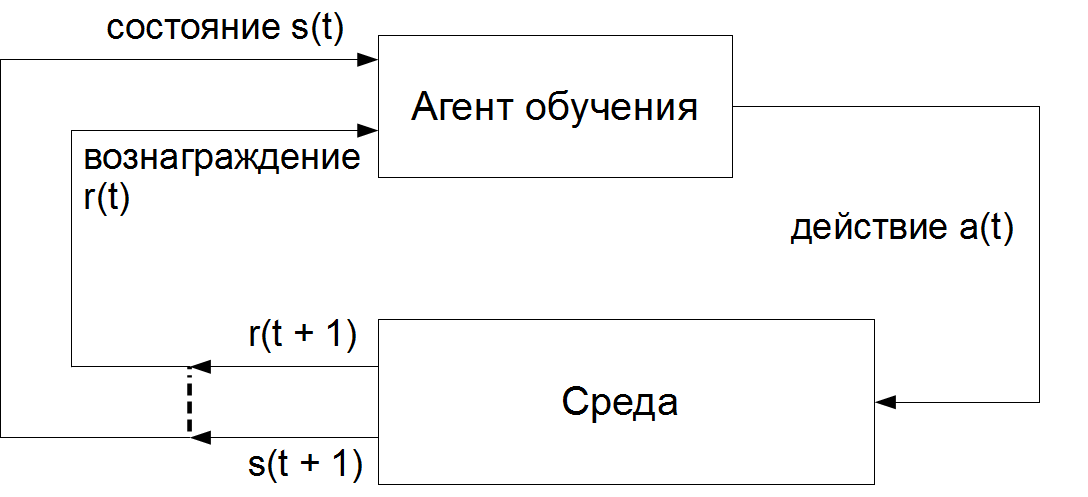
\includegraphics[width=0.6\textwidth]{rl-scheme.png}
    \caption{Схема алгоритма обучения с подкреплением.}
    \label{rl_scheme}
\end{figure}

Принцип работы алгоритма обучения с подкреплением представлен на схеме~\ref{rl_scheme}. Среда находится в некотором состоянии, которое имеет некоторый набор действий. Агент воздействует на среду, выбирая одно из возможных действий и применяя его к среде. В следствие этого среда может перейти в новое состояние. За выбранное действие агент получает награду. Награда выражается вещественнозначным числом. Награда может быть отрицательна в случае штрафа. Задачей агента является максимизация суммарной награды. Действие, выбранное агентом, определяет не только полученную награду, но и состояние, в которое перейдет среда после его применения.

Задачу обучения с подкреплением в большинстве случаев можно описать как \textit{марковский процесс принятия решений}. Для этого необходимо определить:

\begin{itemize}
    \item дискретное множество состояний среды \textit{S};
    \item дискретное множество действий агента \textit{A};
    \item функцию награды $R : S \times A \rightarrow \mathbb{R}$;
    \item функцию переходов $T : S \times A \times S \rightarrow \mathbb{R}$ При этом $T(s, a, s')$ определяет вероятность перехода из состояния $s$ в состояние $s'$ после применения действия $a$.
\end{itemize}

Выделяют класс алгоритмов, которые используют функцию награды \textit{R} и функцию переходов \textit{T} для определения стратегии поведения. В частности, возможны стратегии в которых алгоритм будет получать незначительную награду в течение некоторого времени, чтобы достичь некоторого состояния среды, которому соответствует большая ожидаемая награда. В рамках данной работы такие алгоритмы не рассматривались.

\subsection{Q-обучение}

Алгоритм \textit{Q}-обучения относится к классу алгоритмов обучения с подкреплением не строящих модель среды. Псевдокод алгоритма представлен на листинге~\ref{q_learning}. Во время работы алгоритма аппроксимируется функция полезности $Q : S \times A \rightarrow \mathbb{R}$, которая описывает ожидаемую награду за действие \textit{a} в состоянии \textit{s}. Для расчета значений \textit{Q} обычно используют \textit{TD}-обучение(temporal difference learning). При этом значения \textit{Q} изменяются по формуле $Q(s, a) = Q(s, a) + \alpha (\gamma Q(s', a') - Q(s, a))$, где $\alpha$ -- скорость обучения, $\gamma$ -- дисконтный фактор.

Выбор действия определяется стратегией исследования среды. Одна из самых простых стратегий - \textit{жадная} заключается в том, чтобы выбирать действие, за которое самое большое ожидаемое вознаграждение, т.е. $\argmax\limits_a{\{Q(s, a)\}}$. Однако в таком случае агент склонен выбирать локально максимальное значение награды, недостаточно обследовав среду. Для улучшения жадной стратегии можно выбирать с вероятностью $\epsilon$ случайное действие, иначе -- действие с максимальной ожидаемой наградой. Такая стратегия называется \textit{$\epsilon$-жадной}. При этом значение $\epsilon$ может меняться во время работы алгоритма, что позволяет перейти от исследования среды к применению накопленного опыта.

\begin{algorithm}[h!]
    \caption{Алгоритм Q-обучения с $\varepsilon$-жадной стратегией исследования среды}
    \label{q_learning}
    \begin{algorithmic}[1]
    \REQUIRE  
        $\varepsilon$ --- вероятность выбора случайного действия;
        $\alpha$ --- скорость обучения;
        $\gamma$ --- дисконтный фактор.
    \STATE {Инициализировать $Q(s, a)$ для всех $s \in S$, $a \in A$}
    \WHILE{{(не достигнуто условие останова)}}
        \STATE {Получить состояние среды $s$}
        \STATE $p \gets ${ случайное вещественное число} $\in [0, 1]$
        \IF {($p \leq \varepsilon$)}
            \STATE $a \gets \arg \max_{a}{Q(s,a)}$
        \ELSE 
            \STATE $a \gets$ { случайное действие } $\in A$
        \ENDIF
        \STATE {Применить действие $a$ к среде}
        \STATE {Получить от среды награду $r$ и состояние $s'$}
        \STATE $Q(s,a) \gets Q(s,a) + \alpha(r + \gamma \max_{a'}{Q(s',a') - Q(s, a))}$
    \ENDWHILE
    \end{algorithmic}
\end{algorithm}

\section{Модель UTree}

\subsection{Критерий типа Колмогорова-Смирнова}
\label{ks_criteria}
В статистическом анализе используют различные критерии однородности для проверки гипотезы о принадлежности двух независимых выборок одному закону распределения. Одним из наиболее используемых непараметрических критериев о проверке однородности двух эмпирических законов распределения является критерий однородности Смирнова.

Эмпирическая функция распределения является приближением теоретической функции распределения, построенное с помощью выборки из него. Пусть $\{X_i\}_{i = 1}^n$ выборка из случайной величины $X$, объема $n$. Эмпирической функцией распределения случайной величины $X$ называется случайная величина $F(x) = \frac{1}{n}\sum\limits_{i = 1}^n{H(x - X_i)}$, где $H$~-- функция Хевисайда. По сути заданная таким образом функция распределения в точке $x$ равна частоте элементов выборки, не превосходящих $x$.

\begin{figure}
    \centering
    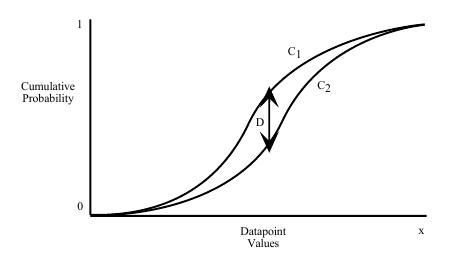
\includegraphics[width=0.6\textwidth]{ks.png}
    \caption{График $F_{a, n}$ и $F_{b, m}$}
    \label{ks}
\end{figure}

Критерий позволяет найти точку, в которой сумма накопленных частот расхождений наибольшая, и оценить достоверность этого расхождения. В качестве нулевой гипотезы $H_0$ принимается, что две исследуемые выборки подчиняются одному закону распределения случайной величины. Для двух независимых выборок $a$ и $b$, объемами $n$ и $m$ соответственно, строятся эмпирические функции распределения $F_{a, n}$ и $F_{b, m}$. Затем считается значение $\sqrt{\frac{nm}{n + m}}D_{n, m}$, где $D_{n, m} = \sup\limits_x|F_{a, n}(x) - F_{b, m}(x)|$. Если рассчитанное значение превышает квантиль распределения Колмогорова $K_{\alpha}$ для заданного уровня значимости $\alpha$, то нулевая гипотеза $H_0$ отвергается.

\section{Метод, предложенный Karafotias}
Метод настройки параметров с помощью обучения с подкреплением.

\section{Метод Earpc}


\section{Модельная задача}

\subsection{Выводы}


\chapter{Предлагаемые методы настройки параметров ЭА}
\label{proposed_chapter}
\section{Цель работы}
Существует метод адаптивной настройки параметров ЭА с помощью обучения с подкреплением, позволяющий адаптивно выделять состояния среды. Множество действий агента определяется разбиением диапазона допустимых значений параметра, которое задается до начала выполнения алгоритма. Также существуют методы настройки параметров ЭА, позволяющие адаптивно разбивать диапазон допустимых значений параметра.

В данной работе предлагается исследовать эффективность адаптивного выделения множества действий агента за счет разбиения диапазона допустимых значений параметра в ходе работы алгоритма. Целью исследований являлась разработка метода адаптивной настройки параметров эволюционного алгоритма с помощью обучения с подкреплением. Предлагаемый алгоритм на основе обучения с подкреплением должен формировать множество действий агента во время работы, адаптивно разбивая диапазон допустимых значений параметра.

\section{Метод на основе алгоритмов EARPC и UTree}
\label{composing_method}
Данный метод является объединением методов \textit{EARPC}~(\ref{earpc}) и \textit{UTree}~(\ref{utree}). В отличие от метода, предложенного Karafotias et al.~(\ref{karafotias}), выбор значений параметров происходит с помощью алгоритма \textit{EARPC}. В процессе работы по наблюдаемым характеристикам ЭА строится дерево решений \textit{UTree}. Алгоритм \textit{EARPC} выбирает значения параметров на основе сохраненных в листе переходов $(I, a, I', r)$. Для оценки качества выбранного назначения параметров для алгоритма \textit{EARPC} используется награда, получаемая агентом. Таким образом, необходимо по наблюдаемым значениям ЭА найти лист дерева \textit{UTree}. Затем значения параметров выбираются при помощи алгоритма \textit{EARPC}, используя переходы, хранящиеся в найденном листе.

При построении дерева \textit{UTree} необходимо определить способ разбиения листа на два состояния. Для применения критерия разбиения Колмогорова-Смирнова, для каждого перехода $(I, a, I', r)$, сохраненного в листе, вычисляется значение $q(I, a) = r + \gamma V(s')$, где $s'$~-- лист, соответствующий характеристикам ЭА $I'$. При этом необходимо посчитать ожидаемую награду $V(s')$. В качестве $V(s')$ предлагается использовать математическое ожидание награды в листе $s'$. Алгоритм \textit{EARPC} разбивает диапазон значений параметра на два подынтервала, один из которых выбирается с вероятностью пропорциональной средней награде на подынтервале. Таким образом $V(s')$ вычисляется по формуле $V(s') = \sum\limits_{i = 1}^2{\frac{Q_i^2}{Q_1 + Q_2}}$, где $Q_1$ и $Q_2$ средние значения награды на первом и втором подынтервале соответственно. 

Кроме того, после выделения новых состояний среды необходимо пересчитать значения ожидаемой награды для полученных состояний. В методе, предложенном \textit{Karafotias et al}., значения $Q(s, a)$, где $s$~-- разбиваемое состояние, копировались в новые состояния, то есть значения ожидаемой награды для полученных состояний не пересчитывались. В предлагаемом подходе при выделении нового состояния в соответствии с алгоритмом \textit{UTree} множество переходов перераспределяется между полученными состояниями. Таким образом значения ожидаемой награды пересчитываются автоматически при следующей итерации алгоритма \textit{EARPC}.

\section{Метод с адаптивным выделением множества действий}
\label{adaptive_method}

Также в данной работе предлагается метод адаптивной настройки параметров ЭА с помощью $Q$-обучения с адаптивным выделением множества действий. В данном подходе действие определяется аналогично методу, предложенному \textit{Karafotias et al}. Однако разбиение диапазона допустимых значений параметров меняется в ходе работы алгоритма.

Агент выбирает действие на основе алгоритма $Q$-обучения с $\varepsilon$-жадной стратегией исследования среды. В случае когда значения ожидаемой награды примерно одинаковы для всех воможных действий, агент не может выбрать какое из действий наиболее эффективно. Поэтому в данном случае текущее разбиение диапазонов значения параметров пересчитывается. При этом в следствие изменения разбиения меняется множество допустимых действий агента.

В процессе работы алгоритма сохраняются выбранные назначения параметров и полученные за эти назначения награды. Сохраненные данные используются при переразбиении диапазона значений для каждого из настраиваемых параметров. Опишем процедуру переразбиения диапазона. Сначала диапазон делится на два подынтервала при помощи критерия Колмогорова-Смирнова. На каждой следующей итерации разбиения диапазона, полученные на текущей итерации подынтервалы при помощи критерия Колмогорова-Смирнова разбиваются на два подынтервала. В случае, если точка разбиения подынтервала не найдена, разбиение интервала не происходит. Таким образом, максимальное число подынтервалов на которые разбивается диапазон допустимых значений параметра равен $2^i$, где $i$~-- число итераций разбиения диапазона. На листинге~\ref{dist_scheme} представлен алгоритм разбиения диапазона для $i = 2$.


\begin{algorithm}[h!]
    \caption{Алгоритм разбиения диапазона с двумя итерациями в методе с адаптивным выделением множества действий.}
    \label{dist_scheme}
    \begin{algorithmic}[1]
	\REQUIRE  
	  \textit{V}~--- множество назначений параметров;
        \FOR {параметр \textit{v}}
	  \STATE {Разбиение $P \gets \emptyset$}
	  \STATE {Отсортировать множество назначений по параметру \textit{v}}
	  \STATE {С помощью критерия Колмогорова-Смирнова найти точку разбиения \textit{s} множества \textit{V}}
	  \IF {Точка разбиения \textit{s} не найдена}
	    \STATE {$P \gets \{[v_{min}, v_{max}]\}$}
	  \ELSE
	    \STATE {Разбить множество \textit{V} на \textit{L} и \textit{R} в соответствии с \textit{s}}
	    \STATE {Найти точку разбиения $s_l$ для множества \textit{L}}
	    \STATE {Найти точку разбиения $s_r$ для множества \textit{R}}
	    \IF {Точки разбиения $s_l$ и $s_r$ не найдены}
	      \STATE {$P \gets \{[v_{min}, s], (s, v_{max}]\}$}
	    \ELSIF {Точка разбиения $s_l$ не найдена}
	      \STATE {$P \gets \{[v_{min}, s], (s, s_r], (s_r, v_{max}]\}$}
	     \ELSIF {Точка разбиения $s_r$ не найдена}
	      \STATE {$P \gets \{[v_{min}, s_l], (s_l, s], (s, v_{max}]\}$}
	     \ELSE
	      \STATE {$P \gets \{[v_{min}, s_l], (s_l, s], (s, s_r], (s_r, v_{max}]\}$}
	    \ENDIF
	  \ENDIF
        \ENDFOR
    \end{algorithmic}
\end{algorithm}

\section{Выводы по главе \protect\ref{proposed_chapter}}
Предложено два метода адаптивной настройки параметров эволюционных алгоритмов с помощью обучения с подкреплением. Оба метода формируют можество действий агента в ходе работы, адаптивно разбивая диапазон допустимых значений настраеваемого параметра. Предложенные подходы являеются достаточно общими и не накладывают ограничения на настраиваемый эволюционный алгоритм.
\printbibliography
\end{document}
